% Options for packages loaded elsewhere
\PassOptionsToPackage{unicode}{hyperref}
\PassOptionsToPackage{hyphens}{url}
\PassOptionsToPackage{dvipsnames,svgnames,x11names}{xcolor}
%
\documentclass[
  english,
  man,floatsintext]{apa6}
\title{Are we all on the same page? Subfield differences in open science practices in psychology}
\author{\phantom{0}}
\date{}

\usepackage{amsmath,amssymb}
\usepackage{lmodern}
\usepackage{iftex}
\ifPDFTeX
  \usepackage[T1]{fontenc}
  \usepackage[utf8]{inputenc}
  \usepackage{textcomp} % provide euro and other symbols
\else % if luatex or xetex
  \usepackage{unicode-math}
  \defaultfontfeatures{Scale=MatchLowercase}
  \defaultfontfeatures[\rmfamily]{Ligatures=TeX,Scale=1}
\fi
% Use upquote if available, for straight quotes in verbatim environments
\IfFileExists{upquote.sty}{\usepackage{upquote}}{}
\IfFileExists{microtype.sty}{% use microtype if available
  \usepackage[]{microtype}
  \UseMicrotypeSet[protrusion]{basicmath} % disable protrusion for tt fonts
}{}
\makeatletter
\@ifundefined{KOMAClassName}{% if non-KOMA class
  \IfFileExists{parskip.sty}{%
    \usepackage{parskip}
  }{% else
    \setlength{\parindent}{0pt}
    \setlength{\parskip}{6pt plus 2pt minus 1pt}}
}{% if KOMA class
  \KOMAoptions{parskip=half}}
\makeatother
\usepackage{xcolor}
\IfFileExists{xurl.sty}{\usepackage{xurl}}{} % add URL line breaks if available
\IfFileExists{bookmark.sty}{\usepackage{bookmark}}{\usepackage{hyperref}}
\hypersetup{
  pdftitle={Are we all on the same page? Subfield differences in open science practices in psychology},
  pdflang={en-EN},
  pdfkeywords={open data; open materials; subfield differences; developmental psychology},
  colorlinks=true,
  linkcolor={Maroon},
  filecolor={Maroon},
  citecolor={Blue},
  urlcolor={blue},
  pdfcreator={LaTeX via pandoc}}
\urlstyle{same} % disable monospaced font for URLs
\usepackage{graphicx}
\makeatletter
\def\maxwidth{\ifdim\Gin@nat@width>\linewidth\linewidth\else\Gin@nat@width\fi}
\def\maxheight{\ifdim\Gin@nat@height>\textheight\textheight\else\Gin@nat@height\fi}
\makeatother
% Scale images if necessary, so that they will not overflow the page
% margins by default, and it is still possible to overwrite the defaults
% using explicit options in \includegraphics[width, height, ...]{}
\setkeys{Gin}{width=\maxwidth,height=\maxheight,keepaspectratio}
% Set default figure placement to htbp
\makeatletter
\def\fps@figure{htbp}
\makeatother
\setlength{\emergencystretch}{3em} % prevent overfull lines
\providecommand{\tightlist}{%
  \setlength{\itemsep}{0pt}\setlength{\parskip}{0pt}}
\setcounter{secnumdepth}{-\maxdimen} % remove section numbering
% Make \paragraph and \subparagraph free-standing
\ifx\paragraph\undefined\else
  \let\oldparagraph\paragraph
  \renewcommand{\paragraph}[1]{\oldparagraph{#1}\mbox{}}
\fi
\ifx\subparagraph\undefined\else
  \let\oldsubparagraph\subparagraph
  \renewcommand{\subparagraph}[1]{\oldsubparagraph{#1}\mbox{}}
\fi
\newlength{\cslhangindent}
\setlength{\cslhangindent}{1.5em}
\newlength{\csllabelwidth}
\setlength{\csllabelwidth}{3em}
\newlength{\cslentryspacingunit} % times entry-spacing
\setlength{\cslentryspacingunit}{\parskip}
\newenvironment{CSLReferences}[2] % #1 hanging-ident, #2 entry spacing
 {% don't indent paragraphs
  \setlength{\parindent}{0pt}
  % turn on hanging indent if param 1 is 1
  \ifodd #1
  \let\oldpar\par
  \def\par{\hangindent=\cslhangindent\oldpar}
  \fi
  % set entry spacing
  \setlength{\parskip}{#2\cslentryspacingunit}
 }%
 {}
\usepackage{calc}
\newcommand{\CSLBlock}[1]{#1\hfill\break}
\newcommand{\CSLLeftMargin}[1]{\parbox[t]{\csllabelwidth}{#1}}
\newcommand{\CSLRightInline}[1]{\parbox[t]{\linewidth - \csllabelwidth}{#1}\break}
\newcommand{\CSLIndent}[1]{\hspace{\cslhangindent}#1}
% Manuscript styling
\usepackage{upgreek}
\captionsetup{font=singlespacing,justification=justified}

% Table formatting
\usepackage{longtable}
\usepackage{lscape}
% \usepackage[counterclockwise]{rotating}   % Landscape page setup for large tables
\usepackage{multirow}		% Table styling
\usepackage{tabularx}		% Control Column width
\usepackage[flushleft]{threeparttable}	% Allows for three part tables with a specified notes section
\usepackage{threeparttablex}            % Lets threeparttable work with longtable

% Create new environments so endfloat can handle them
% \newenvironment{ltable}
%   {\begin{landscape}\centering\begin{threeparttable}}
%   {\end{threeparttable}\end{landscape}}
\newenvironment{lltable}{\begin{landscape}\centering\begin{ThreePartTable}}{\end{ThreePartTable}\end{landscape}}

% Enables adjusting longtable caption width to table width
% Solution found at http://golatex.de/longtable-mit-caption-so-breit-wie-die-tabelle-t15767.html
\makeatletter
\newcommand\LastLTentrywidth{1em}
\newlength\longtablewidth
\setlength{\longtablewidth}{1in}
\newcommand{\getlongtablewidth}{\begingroup \ifcsname LT@\roman{LT@tables}\endcsname \global\longtablewidth=0pt \renewcommand{\LT@entry}[2]{\global\advance\longtablewidth by ##2\relax\gdef\LastLTentrywidth{##2}}\@nameuse{LT@\roman{LT@tables}} \fi \endgroup}

% \setlength{\parindent}{0.5in}
% \setlength{\parskip}{0pt plus 0pt minus 0pt}

% \usepackage{etoolbox}
\makeatletter
\patchcmd{\HyOrg@maketitle}
  {\section{\normalfont\normalsize\abstractname}}
  {\section*{\normalfont\normalsize\abstractname}}
  {}{\typeout{Failed to patch abstract.}}
\patchcmd{\HyOrg@maketitle}
  {\section{\protect\normalfont{\@title}}}
  {\section*{\protect\normalfont{\@title}}}
  {}{\typeout{Failed to patch title.}}
\makeatother
\shorttitle{Subfield differences in open science practices}
\keywords{open data; open materials; subfield differences; developmental psychology\newline\indent Word count: 4748}
\usepackage{lineno}

\linenumbers
\usepackage{csquotes}
\usepackage[titles]{tocloft}
\cftpagenumbersoff{figure}
\renewcommand{\cftfigpresnum}{\itshape\figurename\enspace}
\renewcommand{\cftfigaftersnum}{.\space}
\setlength{\cftfigindent}{0pt}
\setlength{\cftafterloftitleskip}{0pt}
\settowidth{\cftfignumwidth}{Figure 10.\qquad}
\ifXeTeX
  % Load polyglossia as late as possible: uses bidi with RTL langages (e.g. Hebrew, Arabic)
  \usepackage{polyglossia}
  \setmainlanguage[]{english}
\else
  \usepackage[main=english]{babel}
% get rid of language-specific shorthands (see #6817):
\let\LanguageShortHands\languageshorthands
\def\languageshorthands#1{}
\fi
\ifLuaTeX
  \usepackage{selnolig}  % disable illegal ligatures
\fi


\authornote{

Availability Statement: All data, coding and analysis scripts are publicly available via the \href{https://osf.io/z8b7j/?view_only=b97cd4c4f6d645bc9e8870d97b6f3da4}{Open Science Framework repository}. The preregistration can be accessed \href{https://osf.io/gqv9n/?view_only=b97cd4c4f6d645bc9e8870d97b6f3da4}{here}.
Conflict of Interest Disclosure: There were no conflicts of interest in relation to the authorship or publication of this article.
Ethics Approval Statement: The study was approved by the UNSW Human Research Ethics Advisory Panel prior to data collection.
Acknowledgements: The authors would like to acknowledge the tremendous efforts of the coding team (Georgia Saddler, Helen Gu, Jenn Lee, Patrick McCraw, \& Will Osmand). Each member of the coding team played an integral role in this investigation; their assistance is truly appreciated.

}

\affiliation{\phantom{0}}

\abstract{
Although open science has become a popular tool to combat the replication crisis, it is unclear whether the uptake of open science practices has been consistent across the field of psychology. In this study, we tested whether data and material sharing differed as a function of psychological subfield at the distinguished journal, \emph{Psychological Science}. The results showed that open data and open materials scores increased from 2014-2015 to 2019-2020. Of note, articles published in the field of developmental psychology generated lower open data and open materials scores than articles published in cognition, however, scores were similar to articles published in social psychology. Across \emph{Psychological Science} articles, shared data and materials were seldom accompanied by documentation that is likely to make shared research objects useful. These findings are discussed in the context of the unique challenges faces by developmental psychologists and how journals can more effectively encourage authors to practice open science across psychology.
}



\begin{document}
\maketitle

The field of psychology, like many other scientific disciplines, is currently facing a replication crisis, in which researchers are struggling to replicate existing findings. A recent summary of several large scale replication attempts (N = 307 studies total) across psychology reports that only 64\% of studies produced statistically significant effects that were in the same direction as the original published paper (Nosek et al., 2022). These replication studies were highly powered, using samples that were on average 15 times larger than the original study, however, obtained effect sizes that were only 68\% of the original published studies.

Nosek et al., (2022) argue that open science practices may improve replicability by targeting transparency in the research process and making it easier to evaluate the claims made in published work. Open data and open materials practices, for example, involve researchers sharing their raw data and experimental materials on publicly accessible online repositories. Open data and materials can be used to reproduce and verify published results, answer new research questions with existing data, and design replication attempts. These practices are designed to make it easier for others to reproduce the methodology and results from published work (Klein et al., 2018), which may have knock on effects for replicability.

To encourage researchers to employ open science practices, many psychology journals have implemented incentives, like Open Science Badges. In 2013, the Center for Open Science established three Open Science Badges (Open Data, Open Materials and Preregistered) to acknowledge and reward researchers for their use of open science practices (Center for Open Science, 2021). The Open Data and Open Materials Badges, for example, are awarded when the data and materials that are required to reproduce the methods and results of a study are shared publicly online. To date, over 75 journals (40 in Psychology) have adopted Open Science Badges (Center for Open Science, 2021).

At \emph{Psychological Science}, the Association of Psychological Science's flagship journal, Open Science Badges appear to have been successful in encouraging researchers to adopt open science practices. In 2016, Kidwell et al.~coded the frequency of data and material sharing in the 18 months before and after Open Science Badges were implemented at \emph{Psychological Science}. Kidwell et al.~found that data sharing increased dramatically from 2.5\% of articles prior to badges to 39.4\% of articles following badges. Materials sharing also rose from 12.7\% to 30.3\%. Data and material sharing in control journals, such as the \emph{Journal of Personality and Social Psychology}, which did not award badges, remained low over the same time period (Kidwell et al., 2016). Although their study simply described the proportion of articles that engaged in data and materials sharing before and after the policy change, the results led Kidwell et al.~to conclude that Open Science Badges successfully incentivised the uptake of open science practices at \emph{Psychological Science}.

The support for open science continues to grow, however, it is not yet clear whether engagement with open science is consistent across different fields within psychology. Notably, the field of developmental psychology has received significant criticism for its lack of receptivity towards open science. Prominent developmental researchers, Prof Michael Frank and Dr.~Jennifer Pfeifer took to Twitter to label the Society for Research in Child Development's (SRCD) open science policy as `weak' and as one that `undervalues openness.'(Frank, 2020, March 6; Pfeifer, 2020, March 8). More recently, the Editor-in-Chief of Infant and Child Development, Prof Moin Syed, stated that the uptake of open science within the field of developmental psychology has been `slow and uneven' (Syed, 2021). A survey supporting these viewpoints showed that 80\% of researchers publishing in \emph{Child Development} felt their institutions failed to provide adequate guidance or financial support for sharing data (SRCD Task Force on Scientific Integrity and Openness Survey (2017), cited in Gennetian et al., (2020)). Developmental psychology researchers may be slower to adopt open science practices than those in other psychological disciplines, however, this possibility has yet to be empirically investigated.

Using meta-research, the study of research itself, we can empirically assess whether developmental psychology is truly behind in the open science movement. Previous investigations, including Kidwell et al. (2016), have revealed that open science incentives can increase the use of open science practices. However, it is unclear whether Open Science Badges, have had the same impact across different psychological subfields and whether the effect is sustained over time. To address this research question, we used the open data from the Kidwell et al., (2016) study and designed a quantitative scoring system to examine whether rates of data and material sharing following the implementation of Open Science Badges at \emph{Psychological Science}, differed as a function of subfield. In addition, we applied the same coding system to articles published in the most recent 18 months (Jul 2019-Dec 2020) to test whether the badges have continued to be impactful and whether the impact has been consistent across subfields. We were particularly interested in determining whether developmental psychology researchers publishing in \emph{Psychological Science} engaged with open science practices at the same rate as researchers from other subdomains of psychology. Our methods and analysis plan were preregistered at the \href{https://osf.io/gqv9n/?view_only=b97cd4c4f6d645bc9e8870d97b6f3da4}{Open Science Framework}.

\hypertarget{methods}{%
\section{Methods}\label{methods}}

\hypertarget{design}{%
\subsection{Design}\label{design}}

This study had a quasi-experimental design; all articles were systematically assigned to one of seven subfields. For each article, we used coded variables to compute two scores that indexed the transparency of data and materials, respectively.

\hypertarget{sample}{%
\subsection{Sample}\label{sample}}

The Kidwell et al., (2016) sample included all \emph{Psychological Science} articles published between January 2014 and May 2015 (N = 367), which were coded to evaluate the openness of their data and materials. To identify how data and material sharing may have changed since 2014-2015, our sample also included all \emph{Psychological Science} articles that were published between July 2019 and December 2020 (N = 242). Non-empirical articles that did not contain an experiment or analysis, including editorials, commentaries, replies, corrigenda, errata and retractions, were excluded from our analysis. After filtering out these non-empirical articles from the sample, 322 articles published between 2014-2015 and 193 articles published between 2019-2020, remained.

\hypertarget{materials}{%
\subsection{Materials}\label{materials}}

To assess the transparency of data and materials for each article, Kidwell et al.~(2016) employed a systematic coding system (\href{https://osf.io/j4x23/?view_only=b97cd4c4f6d645bc9e8870d97b6f3da4}{Kidwell system} and \href{https://osf.io/n7grj/?view_only=b97cd4c4f6d645bc9e8870d97b6f3da4}{variable definitions}). We downloaded the Kidwell et al.~data from their \href{https://osf.io/rfgdw/}{OSF repository} and filtered the dataset to only include \emph{Psychological Science} articles published between January 2014 and May 2015.

In addition to the variables that Kidwell et al.~had coded, we also coded for whether the article specified their analysis software or not, and which type of analysis software had been specified (e.g., R, JASP, SPSS etc). These variables were important to include because when authors' identify analysis software, the analysis procedure can be easier to follow and the chance of successfully reproducing the analysis may increase (National Academies of Sciences, Medicine, et al., 2019).
The same amended version of the Kidwell et al.~coding system, including the two additional analysis software variables, was used to code the articles that were published between July 2019 and December 2020.

We designed an additional coding system (\href{https://osf.io/a9vgr/?view_only=b97cd4c4f6d645bc9e8870d97b6f3da4}{subfield system} and \href{https://osf.io/md5eu/?view_only=b97cd4c4f6d645bc9e8870d97b6f3da4}{variable definitions}) to assign all the articles to one of seven psychological subfields. Coders answered a series of questions about the type and age participants in the study, the dependent variables, and area of research (see decision tree \url{https://osf.io/a9vgr/}). These variables were used to assign each article to either developmental psychology, social psychology, cognition, perception, health, behavioural neuroscience, or cognitive neuroscience. We identified these seven subfields as those that the majority of \emph{Psychological Science} articles fall into, after thoroughly reviewing the journal website.

Prior to data collection, each member of the coding team coded five trial articles, to confirm their understanding of the coding process. These trial articles were \emph{Psychological Science} articles originally coded by Mallory Kidwell, the primary investigator in the Kidwell et al.~(2016) study. Kidwell's coding acted as the standard to which coders' responses were compared. The senior coder in the current study generated the standard for the variables that weren't included in the Kidwell et al.~coding system (i.e.~those related to software and subfield). The trial articles varied in the transparency of their data and materials, and therefore, exposed coders to a representative range of coding outcomes.

The coding team coded both the trial and target articles via a Qualtrics survey, containing a series of multiple-choice questions. The questions were structured in an `if-then' manner, with some questions only being asked if coders provided particular answers to the questions prior. For example, coders were only asked about the participants' age, if they had specified that the participants in the study were `Humans' rather than `Animals.'

\hypertarget{procedure}{%
\subsection{Procedure}\label{procedure}}

After the investigation had been approved by the Human Research Ethics Advisory Panel, we assembled a team of volunteer coders, comprising of undergraduate psychology students. Once the coders completed the five trial articles and the senior coder was confident that each coder understood how to code all the variables, the coders were provided access to the target set of articles to begin coding using the Qualtrics survey.

\hypertarget{scoring-procedure}{%
\subsubsection{Scoring procedure}\label{scoring-procedure}}

After all articles had been coded, we imported the data from Qualtrics into the software environment, R (R Core Team, 2020). For the articles that were published between 2014-2015, we combined the newly collected data related to softwre and subfield with the data from Kidwell et al.~(2016). Each article, across both the 2014-2015 and 2019-2020 datasets, was assigned to one of the seven psychological subfields and received an open data and open materials score. The open data score indexed the extent to which the data were transparent, whilst the open materials score indexed the extent to which the materials were transparent.

\emph{Table 1}: Open data scoring (left) and open materials scoring (right) criteria

\begin{figure}

{\centering 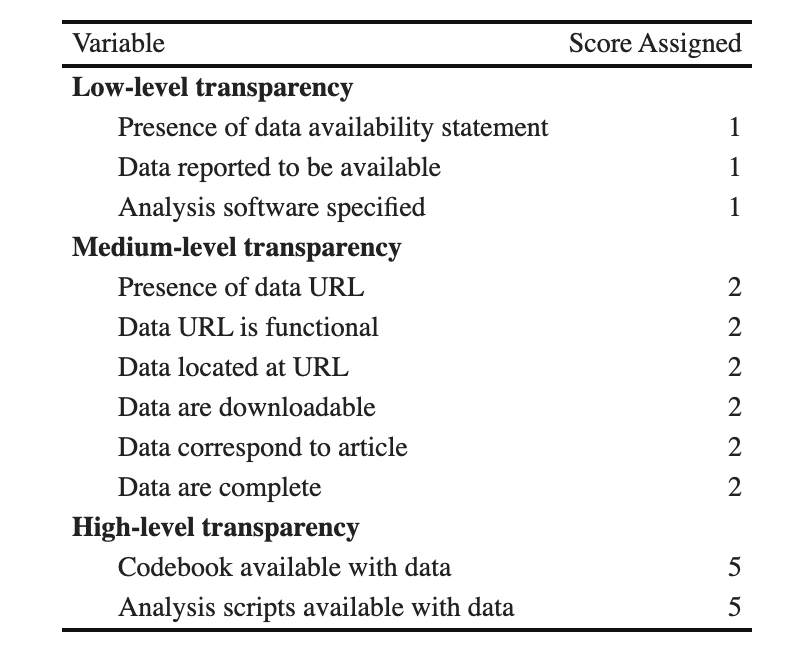
\includegraphics[width=0.49\linewidth,height=0.2\textheight]{data_scoring} 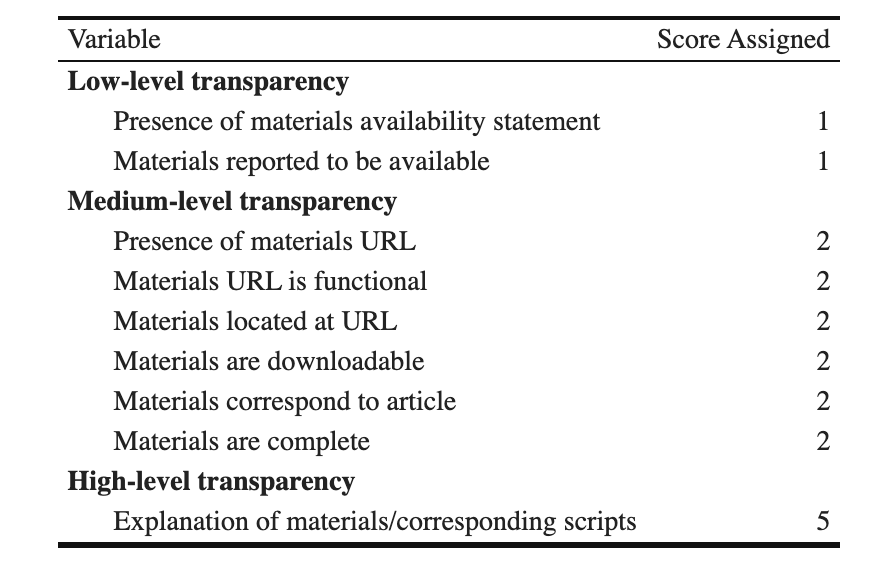
\includegraphics[width=0.49\linewidth,height=0.2\textheight]{mat_scoring} 

}

\end{figure}

To calculate the scores, we weighted each coded variable according to the additional effort required to engage in that behaviour. There were three levels of transparency (see Table 1). Low-level transparency variables (1 point) require only a line of text to be included in the manuscript. Moderate-level transparency variables (2 points) are the minimum required to earn an open data/materials badge. High-level transparency variables (5 points) require additional effort outside of common research workflow and represent best practice. We summed these scores so that each article received an open data score out of a possible 25 and an open materials score out of a possible 19. Open data and materials scores were scaled by dividing each score by the maximum; both are presented on a scale from 0 - 1. Scores closer to 1 reflect a higher level of transparency.

\hypertarget{reliability}{%
\subsubsection{Reliability}\label{reliability}}

The senior coder randomly selected 25 empirical articles from the 2014-2015 dataset (8\% of the empirical sample), ensuring that an equal number had been coded by each coder (n = 5), and double-coded these software and subfield variable. Using the `kappa2' function from the `irr' package in R (Gamer, Lemon, \& Singh, 2019), we ran a Cohen's Kappa reliability analysis for subfield assignment, which revealed that the coding team had good reliability compared to the senior coder's standard, k = .605, according to Fleiss's (1981) guidelines. The percent agreement rating between the standard and the coding team was 72\%. Upon examining cases where the standard and the coding team disagreed on an article's subfield assignment, we found that the discrepancy could usually be attributed to the subject matter spanning across multiple subfields. Since our coding system did not account for the possibility of a study belonging to multiple subfields, the results from our reliability analysis may be conservative.

For the 2019-2020 sample of articles, the senior coder similarly selected 25 articles from the empirical sample (13\%) and double-coded these articles. To assess reliability, each article received a total openness score, representing the sum of the open data and open materials score. We used the `icc' function from the `irr' package in R to generate an intraclass correlation coefficient (ICC) (Gamer et al., 2019). The `tolerance' level was set at five Total Openness points; where scores fell within a five-point range of each other, they were considered to be equivalent.

The ICC analysis showed that the coding team had excellent reliability relative to the senior coder's standard, according to Cicchetti's (1994) guidelines, ICC = .905, 95\% CI (.772, .962). As a secondary measure of inter-rater reliability, we also calculated the percent agreement between the standard and coders' responses. The agreement rating between the coders and the standard was 73.7\%, with a tolerance level of five Total Openness points.

\hypertarget{data-analysis}{%
\subsubsection{Data analysis}\label{data-analysis}}

We used R {[}Version 4.1.1; R Core Team (2020){]} and the R-packages \emph{afex} {[}Version 1.1.1; Singmann, Bolker, Westfall, Aust, and Ben-Shachar (2021){]}, \emph{apa} {[}Version 0.3.3; Gromer (2020); Aust and Barth (2020){]}, \emph{dplyr} {[}Version 1.0.9; Wickham, François, Henry, and Müller (2021){]}, \emph{forcats} {[}Version 0.5.1; Wickham (2021a){]}, \emph{ggeasy} {[}Version 0.1.3; Carroll, Schep, and Sidi (2021){]}, \emph{gghalves} {[}Version 0.1.1; Tiedemann (2020){]}, \emph{ggplot2} {[}Version 3.3.6; Wickham (2016){]}, \emph{ggsankey} {[}Version 0.0.99999; Sjoberg (2022){]}, \emph{ggsignif} {[}Version 0.6.3; Constantin and Patil (2021){]}, \emph{goodshirt} (Gruer, 2021), \emph{gt} {[}Version 0.6.0; Iannone, Cheng, and Schloerke (2022){]}, \emph{here} {[}Version 1.0.1; Müller (2020){]}, \emph{irr} (Gamer et al., 2019), \emph{janitor} {[}Version 2.1.0; Firke (2021){]}, \emph{kableExtra} {[}Version 1.3.4; Zhu (2021){]}, \emph{lme4} {[}Version 1.1.29; Bates, Mächler, Bolker, and Walker (2015){]}, \emph{Matrix} {[}Version 1.4.1; Bates and Maechler (2021){]}, \emph{papaja} {[}Version 0.1.0.9997; Aust and Barth (2020){]}, \emph{patchwork} {[}Version 1.1.1; Pedersen (2020){]}, \emph{purrr} {[}Version 0.3.4; Henry and Wickham (2020){]}, \emph{readr} {[}Version 2.1.2; Wickham and Hester (2021){]}, \emph{report} (Makowski, Ben-Shachar, Patil, \& Lüdecke, 2021), \emph{scales} {[}Version 1.2.0; Wickham and Seidel (2020){]}, \emph{stringr} {[}Version 1.4.0; Wickham (2019){]}, \emph{tibble} {[}Version 3.1.7; Müller and Wickham (2021){]}, \emph{tidyr} {[}Version 1.2.0; Wickham (2021b){]}, and \emph{tidyverse} {[}Version 1.3.1; Wickham et al. (2019){]} for all our analyses.

We preregistered our aims, hypotheses, design, and planned analysis procedure for the study at the \href{https://osf.io/gqv9n/?view_only=b97cd4c4f6d645bc9e8870d97b6f3da4}{OSF}, planning to compare differences in open data and open materials scores across the 2014-2015 and 2019-2020, as a function of subfield.
As anticipated in our preregistration, articles were not evenly distributed across all 7 subfield categories (see Table 1 and 2 supplementary materials). Given that 77\% of 2014-15 articles and 79\% of 2019-2020 articles fell into either cognition, social psychology or developmental psychology categories, we decided to combine articles in the remaining categories (Cognitive Neuroscience, Behavioural Neuroscience, Health Psychology and Perception) into a single `Other' category. As a result, a total of four subfield groups were included in our analysis: Developmental Psychology, Social Psychology, Cognition and Other.

Whilst we attempted to follow each of the proposed procedures as closely as possible, following feedback from reviewers, we decided that inferential statistics were not necessary to answer the research question and were inappropriate given the bimodal of the data. The final analyses reported here are exploratory and focused on descriptives. All the materials, data and analysis scripts from the study can be accessed via the \href{https://osf.io/z8b7j/?view_only=b97cd4c4f6d645bc9e8870d97b6f3da4}{OSF}.

After data collection, we explored the distribution of scores and how the spread of scores might differ by subfield. To illustrate this we generated two raincloud plots that illustrated the distribution of open data and open materials scores across 2019-2020. Raincloud plots visualise the distribution of scores in a dataset by showing the density of subjects at each level of the dependent measure (Allen, Poggiali, Whitaker, Marshall, \& Kievit, 2019). In our case, where the violin plot was wider, the concentration of articles that received the corresponding open data or open materials score, was greater.

We also wanted to learn how Open Science Badges related to researchers' data and materials sharing practices. To generate two corresponding figures, we filtered the 2019-2020 dataset to only include the articles that had received an Open Data Badge and an Open Materials Badge, respectively. We then plotted the percentage of these articles that met a series of data and materials sharing criteria, described in the Results section below.

\hypertarget{results}{%
\section{Results}\label{results}}

We first used the open data from Kidwell et al., (2016) and analysed whether open data and open materials scores improved across the 2014-2015 period and differed by subfield. As illustrated in Figure 1A, during the period immediately following the badge policy change, open data scores were uniformly low across subfields.

\begin{figure}
\centering
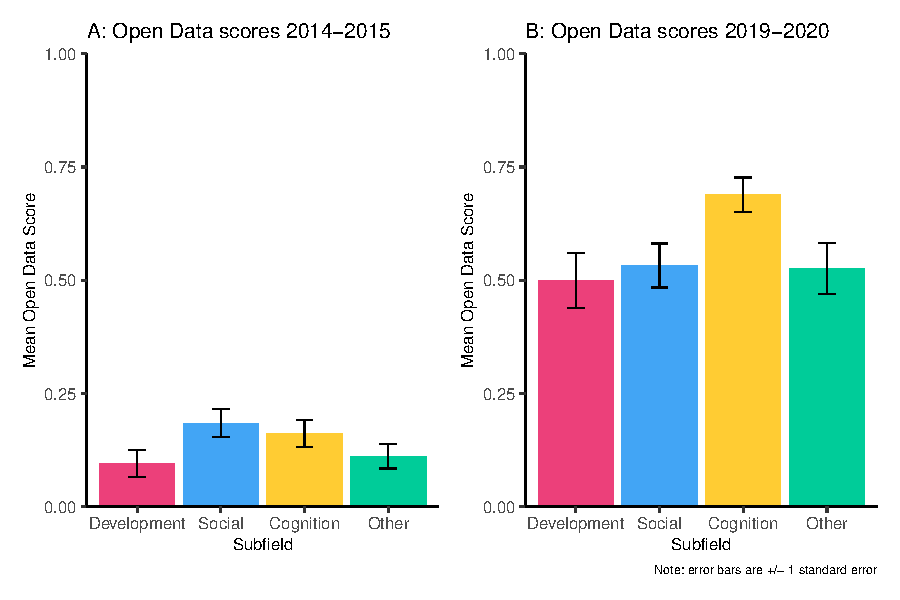
\includegraphics{icd_special_issue_revision_files/figure-latex/unnamed-chunk-2-1.pdf}
\caption{\label{fig:unnamed-chunk-2}Mean open data scores for articles published in \emph{Psychological Science} between 2014-2015 and 2019-2020 as a function of subfield.}
\end{figure}

When we summarised mean open data scores from papers published in 2019-2020 as a function of subfield we saw that scores had improved markedly (see Figure 1B). Cognition papers had highest open data scores (\emph{M} = 0.69, \emph{SD} = 0.29), however, papers in development (\emph{M} = 0.50, \emph{SD} = 0.35) had open data scores that were similar to social psychology (\emph{M} = 0.53, \emph{SD} = 0.37) and those that fell into the other category (\emph{M} = 0.53, \emph{SD} = 0.36).

\begin{figure}
\centering
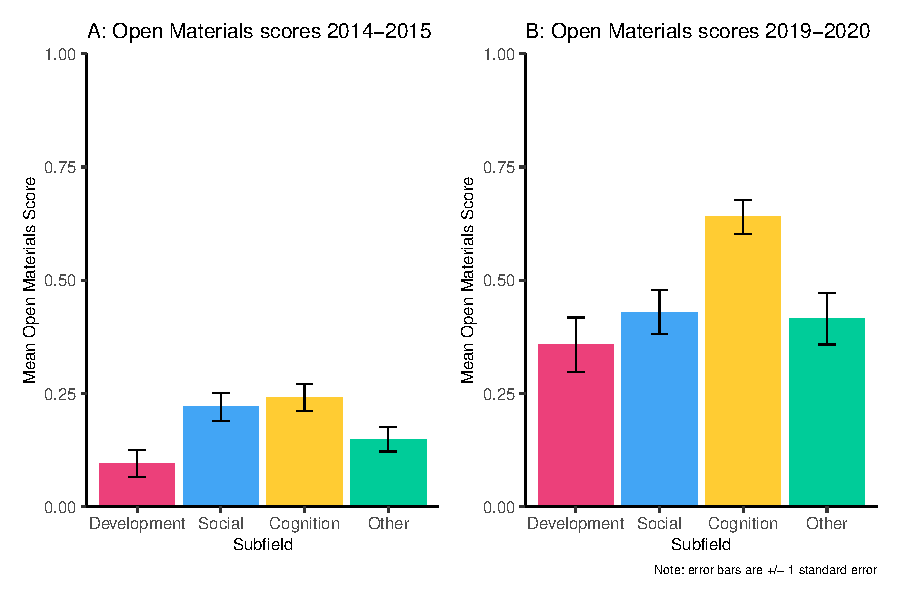
\includegraphics{icd_special_issue_revision_files/figure-latex/unnamed-chunk-3-1.pdf}
\caption{\label{fig:unnamed-chunk-3}Mean open materials scores for articles published in \emph{Psychological Science} between 2014-2015 and 2019-2020 as a function of subfield.}
\end{figure}

A similar pattern was seen for open materials scores (as illustrated in Figure 2A and 2B). For open materials scores across 2014-2015, papers in developmental psychology had open materials scores (\emph{M} = 0.10, \emph{SD} = 0.24) that were somewhat lower than those in both social (\emph{M} = 0.22, \emph{SD} = 0.29) and cognition categories (\emph{M} = 0.24, \emph{SD} = 0.28). Open materials scores were again markedly higher during the 2019-2020 period (see Figure 2B), however, papers published in developmental psychology and social psychology had continued to have lower open materials scores (\emph{M} = 0.36, \emph{SD} = 0.35) than papers published in cognition, (\emph{M} = 0.36, \emph{SD} = 0.35). It is clear that since the introduction of Open Science Badges in 2014, papers published in \emph{Psychological Science} have become more open over time and that most recently, developmental psychology has lagged behind cognition but not other subfields.

\begin{figure}
\centering
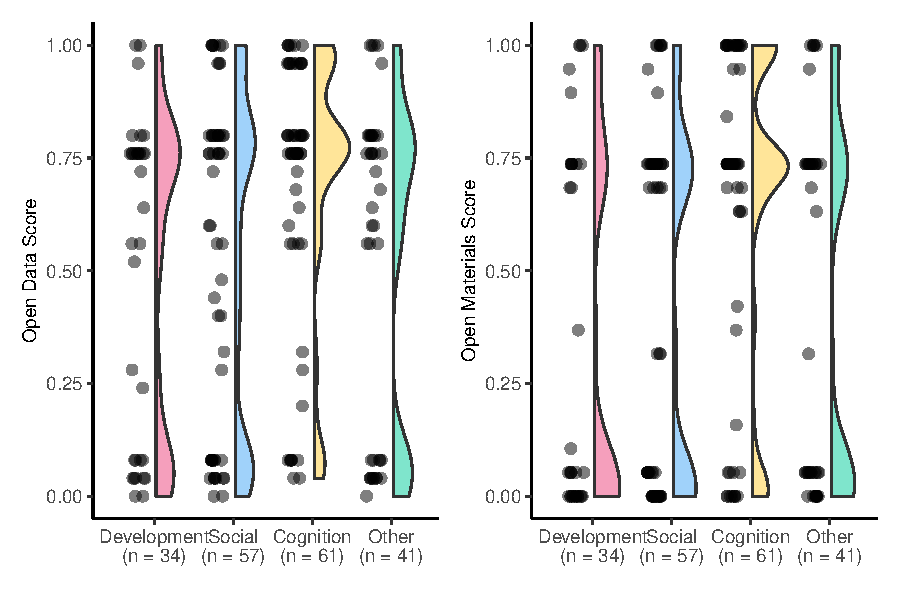
\includegraphics{icd_special_issue_revision_files/figure-latex/rain-1.pdf}
\caption{\label{fig:rain}Distribution of open data and open materials scores earned by articles published in \emph{Psychological Science} between 2019 and 2020 as a function of subfield}
\end{figure}

Our analyses show that on average, open data and materials scores for papers published in \emph{Psychological Science} have increased markedly across all subfields, however, scores within each subfield varied widely. To explore this variability, we used raincloud plots (Allen et al., 2019) to represent the distribution of open data and materials scores across subfields. Figure 3 illustrates that the majority of papers score on the upper half of the scale, however, there are still one third of papers published that receive scores less than 0.25.

\begin{figure}
\centering
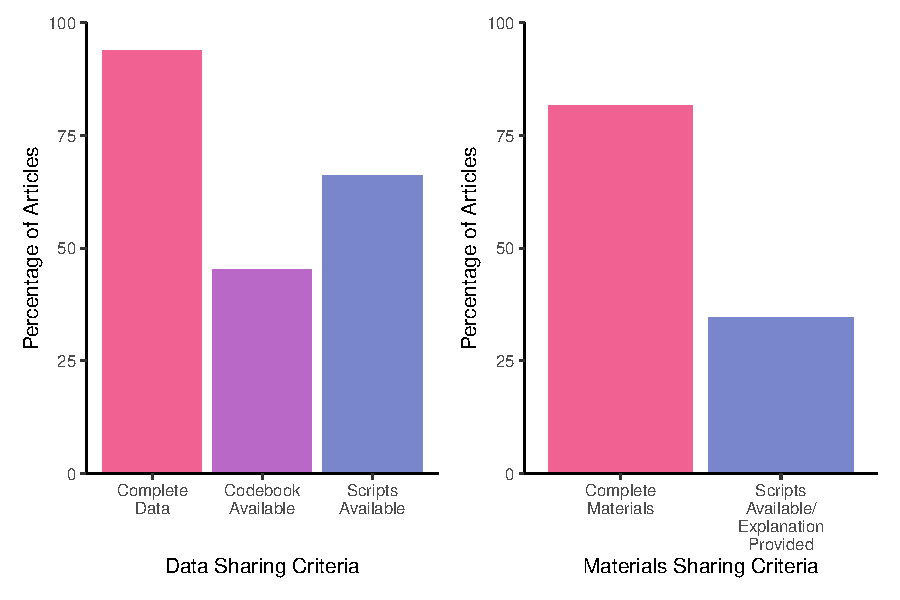
\includegraphics{icd_special_issue_revision_files/figure-latex/unnamed-chunk-4-1.pdf}
\caption{\label{fig:unnamed-chunk-4}Proportion of articles published in \emph{Psychological Science} in 2019-2020 that earned an Open Data Badge (left) or Open Materials Badge (right) and engaged with sharing criteria behaviours}
\end{figure}

We were surprised how few articles received very high open data and materials scores even in 2019-2020. In order to receive very high scores, authors needed to engage in behaviours that make shared resources more likely to be useful (i.e.~sharing data with a accompanying codebook and analysis script). We were particularly interested in how common this kind of metadata sharing was among papers that had earned an Open Data or Open Materials Badge. To produce Figure 4, we filtered articles published within the 2019-2020 window for those that were awarded open data and materials badges and then plotted the proportion of those articles that shared codebooks and scripts along with complete data.

Figure 4 shows that the vast majority of papers earning an open data badge had complete data available, however, less than half shared a codebook and only 66\% included an analysis script. Similarly for open materials, most articles earning a badge shared raw materials on an open repository, but a relatively small percentage of articles also shared an script and/or detailed explanation of how to use the materials in a replication study.

\hypertarget{discussion}{%
\section{Discussion}\label{discussion}}

In the past few years, there has been concern from some academics that developmental psychology was lagging behind in its use of open science practices, compared to other psychological subfields. Our analysis showed that since the introduction of Open Science Badges at \emph{Psychological Science} in 2014, open science practices have improved across the board. While developmental psychology articles published in \emph{Psychological Science} most recently had lower open data and open materials scores than cognition articles, scores were no lower than social psychology articles. As such, Wwe found no evidence that developmental psychology was generally lagging behind.

There are several factors that may be contributing to lower open data and open materials scores in developmental psychology relative to cognitive psychology. Notably, practicing open science may pose a greater reputational risk to developmental scientists compared to researchers from other subdisciplines (Gilmore, Cole, Verma, Van Aken, \& Worthman, 2020). Participants in developmental research are temperamental and unpredictable, which makes it difficult for researchers to stick to strict experimental protocols (Peterson, 2016). For example, if a child is getting fussy, the experimenter may deviate from the experimental protocol and allow the parent to complete the paradigm with them (Slaughter \& Suddendorf, 2007). These ``off-protocol'' decisions make protocols difficult to reproduce and add noise to experimental data (Peterson, 2016). Researchers may be reluctant to share data and materials openly, out of fear that those materials and data will be scrutinised and found to lack scientific rigor (Gilmore et al., 2020). It is possible that the perceived reputational risks of data and material sharing in developmental psychology may impact openness and transparency.

The scarcity of data in developmental psychology may further impede data sharing. Developmental scientists usually recruit their participants from off-campus locations (Peterson, 2016) making recruitment a time consuming and expensive process and sample sizes generally small (Davis-Kean \& Ellis, 2019). In contrast, cognition researchers are typically able to recruit large samples of participants on campus or from online platforms (Benjamin, 2019). According to the law of supply and demand, rare commodities are more highly valued (Steuart, 1767). Given that willingness to share decreases as the value of an item increases (Hellwig, Morhart, Girardin, \& Hauser, 2015) it is possible that developmental researchers are less likely to share data simply because it is more highly valued.

Finally, the methods that developmental psychologists use may make it particularly difficult to share materials openly. As Peterson (2016) reports, in developmental studies, experimental stimuli are typically constructed by hand and are set up manually by research assistants. The physical nature of these experimental paradigms may make them more difficult, and sometimes impossible, to share online. In contrast, computer-based experimental paradigms are becoming increasingly popular in cognition. These paradigms, which can be automated and run online, make it relatively easy to upload materials to online repositories (Paxton \& Tullett, 2019). Subfield differences in the types of materials researchers employ may explain why developmental psychologists are less likely to share materials than researchers in cognition, for example.

Although open data and materials sharing may be more challenging for developmental psychology researchers, there is cause for optimism. Open data and materials scores for developmental psychology articles published in \emph{Psychological Science} improved from 2014 to 2020 at the same rate as articles in other subfields. It seems that developmental psychology researchers, at least those who are looking to publish in \emph{Psychological Science}, are keeping up with their colleagues and becoming more and more likely to adopt open data and open materials into their research workflow.

It is clear that open data and materials practices are becoming more common, however, the current findings highlight the significant progress that has yet to be made in the open science movement across the field of psychology. We were surprised to see that in 2019-2020 a large proportion of articles received extremely low scores open data and open materials scores. In addition, very few articles were awarded the highest possible open data and open materials score, indicating that even when data and materials were shared, they were often not accompanied by a codebook, analysis script and/or explanation of the materials. Roche et al. (2015) suggest that without these metadata, open data and open materials may not be usable, both for the purpose of reproducing the findings of a particular study and conducting novel research. Recent attempts to reproduce results from a small subset (N= 25) studies published in \emph{Psychological Science} have shown that without communication with the authors, results from fewer than 40\% of papers were reproducible (Hardwicke et al., 2021). Unfortunately, only 6 of the papers in this sample included an analysis script, making it difficult to know whether articles that share an codebook and/or analysis script are more reproducible than articles that do not share additional metadata.

Like all open science incentives, Open Science Badges are not an end to themselves. Incentives like badges are designed to improve the transparency of research methods, which may make research more reproducable, and ultimately more replicable (Nosek et al., 2022). Whilst Open Science Badges appear to incentivise researchers to share their data and materials, if they do not increase the availability of metadata, which allows others to use the data to evaluate the claims made in published work, then the value of open badges in addressing the replication crisis remains in doubt.

Our results also raise concerns about how well Open Science Badges criteria are adhered to, in practice. According to the COS, Open Data Badges can only be awarded if a `data dictionary' such as a codebook, or other related metadata is made available (Center for Open Science, 2013a). Similarly, for articles to be awarded an Open Materials Badge, the authors must provide a sufficiently detailed explanation of how the materials were used in the study, and how they can be reproduced, if they can't be shared digitally (Center for Open Science, 2013b). We found that only 45\% of the articles that were awarded an Open Data Badge in 2019-2020, shared a codebook, and only 35\% of those awarded an Open Materials Badge provided an explanation of their materials. These results not only suggest that a very small proportion of the articles that received an Open Data and/or Open Materials Badge were truly deserving of one, but they also show that the criteria for Open Science Badges may be applied inconsistently. Further research is required to identify whether this issue is specific to \emph{Psychological Science}, or if it is a broader issue observed across all journals that award Open Science Badges. In any case, the potentially inconsistent application of the criteria for Open Science Badges questions how valid and reliable they are as indicators of transparency and usability.

Although \emph{Psychological Science} was ideally suited for our subfield comparison due to its broad publishing scope, the results reported here may not generalise to psychology research broadly. In restricting our analysis to articles published in \emph{Psychological Science}, we have coded a very small subset of high quality and novel research articles. It is possible that open science researchers are over-represented among researchers who are drawn to \emph{Psychological Science} as a publishing outlet. Alternatively, it is possible that the improvements we have seen at \emph{Psychological Science} reflect a broader field-wide shift in research workflow, rather than the effect of badges per se. Future meta-research should focus on the impact of incentivising open science practices across a broader range of psychology journals.

Although Open Science Badges may encourage authors to be more transparent in their research, it is possible that they are rewarding researchers for doing the bare minimum, and not actually pushing the field toward a more reproducible and ultimately replicable science. It is possible that an open science scoring system could encourage researchers to share their data and materials in a way that makes them useful to others. Such a system (see (Hartshorne \& Schachner, 2012; Yang, Youyou, \& Uzzi, 2020) for related examples) would involve psychology journals awarding each article they publish a ``Reproduciblity Score'' that indexes the likelihood of the findings being successfully reproduced based on the transparency of the data and materials. To maximise objectivity and to minimise time costs, an automated algorithm would generate the Reproducibility Score (Altmejd et al., 2019; Yang et al., 2020). Future research should test whether scores may be a more precise and meaningful indicator of transparency, reproducibility, and potential replicability.

The present study shows that developmental psychology researchers are improving in their use of open science practices, however, the frequency of behaviours that promote reproducibility are surprisingly uncommon across papers published in \emph{Psychological Science}. It may be that a scoring system could provide more specific incentives that encourage researchers to go beyond what is required to earn an open science badge, and engage in behaviours that make their data useful to others.

\newpage

\hypertarget{references}{%
\section{References}\label{references}}

\begingroup
\setlength{\parindent}{-0.5in}
\setlength{\leftskip}{0.5in}

\hypertarget{refs}{}
\begin{CSLReferences}{1}{0}
\leavevmode\vadjust pre{\hypertarget{ref-allen2019raincloud}{}}%
Allen, M., Poggiali, D., Whitaker, K., Marshall, T. R., \& Kievit, R. A. (2019). Raincloud plots: A multi-platform tool for robust data visualization. \emph{Wellcome Open Research}, \emph{4}. \url{https://doi.org/10.12688/wellcomeopenres.15191.1}

\leavevmode\vadjust pre{\hypertarget{ref-altmejd2019predicting}{}}%
Altmejd, A., Dreber, A., Forsell, E., Huber, J., Imai, T., Johannesson, M., \ldots{} Camerer, C. (2019). Predicting the replicability of social science lab experiments. \emph{PloS One}, \emph{14}(12), e0225826. \url{https://doi.org/10.1371/journal.pone.0225826}

\leavevmode\vadjust pre{\hypertarget{ref-R-papaja}{}}%
Aust, F., \& Barth, M. (2020). \emph{{papaja}: {Create} {APA} manuscripts with {R Markdown}}. Retrieved from \url{https://github.com/crsh/papaja}

\leavevmode\vadjust pre{\hypertarget{ref-R-lme4}{}}%
Bates, D., Mächler, M., Bolker, B., \& Walker, S. (2015). Fitting linear mixed-effects models using {lme4}. \emph{Journal of Statistical Software}, \emph{67}(1), 1--48. \url{https://doi.org/10.18637/jss.v067.i01}

\leavevmode\vadjust pre{\hypertarget{ref-R-Matrix}{}}%
Bates, D., \& Maechler, M. (2021). \emph{Matrix: Sparse and dense matrix classes and methods}. Retrieved from \url{https://CRAN.R-project.org/package=Matrix}

\leavevmode\vadjust pre{\hypertarget{ref-benjamin2019}{}}%
Benjamin, A. S. (2019). Editorial. \emph{Journal of Experimental Psychology: Learning, Memory, and Cognition}, \emph{45}(2). \url{https://doi.org/10.1037/xlm0000688}

\leavevmode\vadjust pre{\hypertarget{ref-R-ggeasy}{}}%
Carroll, J., Schep, A., \& Sidi, J. (2021). \emph{Ggeasy: Easy access to 'ggplot2' commands}. Retrieved from \url{https://CRAN.R-project.org/package=ggeasy}

\leavevmode\vadjust pre{\hypertarget{ref-center_2013a}{}}%
Center for Open Science. (2013a). Open data badge criteria. Retrieved from \url{https://osf.io/g6u5k/}

\leavevmode\vadjust pre{\hypertarget{ref-center_2013b}{}}%
Center for Open Science. (2013b). Open materials badge criteria. Retrieved from \url{https://osf.io/gc2g8/}

\leavevmode\vadjust pre{\hypertarget{ref-cicchetti1994guidelines}{}}%
Cicchetti, D. V. (1994). Guidelines, criteria, and rules of thumb for evaluating normed and standardized assessment instruments in psychology. \emph{Psychological Assessment}, \emph{6}(4), 284. \url{https://doi.org/10.1037/1040-3590.6.4.284}

\leavevmode\vadjust pre{\hypertarget{ref-R-ggsignif}{}}%
Constantin, A.-E., \& Patil, I. (2021). {ggsignif}: R package for displaying significance brackets for {'ggplot2'}. \emph{PsyArxiv}. \url{https://doi.org/10.31234/osf.io/7awm6}

\leavevmode\vadjust pre{\hypertarget{ref-davis2019overview}{}}%
Davis-Kean, P. E., \& Ellis, A. (2019). An overview of issues in infant and developmental research for the creation of robust and replicable science. \emph{Infant Behavior and Development}, \emph{57}, 101339. \url{https://doi.org/10.1016/j.infbeh.2019.101339}

\leavevmode\vadjust pre{\hypertarget{ref-R-janitor}{}}%
Firke, S. (2021). \emph{Janitor: Simple tools for examining and cleaning dirty data}. Retrieved from \url{https://CRAN.R-project.org/package=janitor}

\leavevmode\vadjust pre{\hypertarget{ref-fleiss1981balanced}{}}%
Fleiss, J. L. (1981). Balanced incomplete block designs for inter-rater reliability studies. \emph{Applied Psychological Measurement}, \emph{5}(1), 105--112. \url{https://doi.org/10.1177/014662168100500115}

\leavevmode\vadjust pre{\hypertarget{ref-Frank_tweet}{}}%
Frank, M. {[}@mcxfrank{]}. (2020, March 6). At the same time, this policy statement is weaker than it should be! Openness does not just cause harm. It also reduces harm - often dramatically {[}tweet{]}. Retrieved from \url{https://twitter.com/mcxfrank/status/1103068416791855104}

\leavevmode\vadjust pre{\hypertarget{ref-R-irr}{}}%
Gamer, M., Lemon, J., \& Singh, I. F. P. (2019). \emph{Irr: Various coefficients of interrater reliability and agreement}. Retrieved from \url{https://CRAN.R-project.org/package=irr}

\leavevmode\vadjust pre{\hypertarget{ref-gennetian2020advancing}{}}%
Gennetian, L. A., Tamis-LeMonda, C. S., \& Frank, M. C. (2020). Advancing transparency and openness in child development research: opportunities. \emph{Child Development Perspectives}, \emph{14}(1), 3--8. \url{https://doi.org/10.1111/cdep.12356}

\leavevmode\vadjust pre{\hypertarget{ref-gilmore2020advancing}{}}%
Gilmore, R. O., Cole, P. M., Verma, S., Van Aken, M. A., \& Worthman, C. M. (2020). Advancing scientific integrity, transparency, and openness in child development research: Challenges and possible solutions. \emph{Child Development Perspectives}, \emph{14}(1), 9--14. \url{https://doi.org/10.1111/cdep.12360}

\leavevmode\vadjust pre{\hypertarget{ref-R-apa}{}}%
Gromer, D. (2020). \emph{Apa: Format outputs of statistical tests according to APA guidelines}. Retrieved from \url{https://CRAN.R-project.org/package=apa}

\leavevmode\vadjust pre{\hypertarget{ref-R-goodshirt}{}}%
Gruer, A. (2021). \emph{Goodshirt: R client for the good place quotes API}.

\leavevmode\vadjust pre{\hypertarget{ref-hardwicke2021analytic}{}}%
Hardwicke, T. E., Bohn, M., MacDonald, K., Hembacher, E., Nuijten, M. B., Peloquin, B. N., \ldots{} Frank, M. C. (2021). Analytic reproducibility in articles receiving open data badges at the journal psychological science: An observational study.

\leavevmode\vadjust pre{\hypertarget{ref-hartshorne2012tracking}{}}%
Hartshorne, J., \& Schachner, A. (2012). Tracking replicability as a method of post-publication open evaluation. \emph{Frontiers in Computational Neuroscience}, \emph{6}, 8. \url{https://doi.org/10.3389/fncom.2012.00008}

\leavevmode\vadjust pre{\hypertarget{ref-hellwig2015exploring}{}}%
Hellwig, K., Morhart, F., Girardin, F., \& Hauser, M. (2015). Exploring different types of sharing: A proposed segmentation of the market for {``sharing''} businesses. \emph{Psychology \& Marketing}, \emph{32}(9), 891--906. \url{https://doi.org/10.1002/mar.20825}

\leavevmode\vadjust pre{\hypertarget{ref-R-purrr}{}}%
Henry, L., \& Wickham, H. (2020). \emph{Purrr: Functional programming tools}. Retrieved from \url{https://CRAN.R-project.org/package=purrr}

\leavevmode\vadjust pre{\hypertarget{ref-R-gt}{}}%
Iannone, R., Cheng, J., \& Schloerke, B. (2022). \emph{Gt: Easily create presentation-ready display tables}. Retrieved from \url{https://CRAN.R-project.org/package=gt}

\leavevmode\vadjust pre{\hypertarget{ref-kidwell2016badges}{}}%
Kidwell, M. C., Lazarević, L. B., Baranski, E., Hardwicke, T. E., Piechowski, S., Falkenberg, L.-S., \ldots{} others. (2016). Badges to acknowledge open practices: A simple, low-cost, effective method for increasing transparency. \emph{PLoS Biology}, \emph{14}(5), e1002456. \url{https://doi.org/10.1371/journal.pbio.1002456}

\leavevmode\vadjust pre{\hypertarget{ref-klein2018practical}{}}%
Klein, O., Hardwicke, T. E., Aust, F., Breuer, J., Danielsson, H., Mohr, A. H., \ldots{} others. (2018). A practical guide for transparency in psychological science. \emph{Collabra: Psychology}, \emph{4}(1). \url{https://doi.org/10.1525/collabra.158}

\leavevmode\vadjust pre{\hypertarget{ref-R-report}{}}%
Makowski, D., Ben-Shachar, M. S., Patil, I., \& Lüdecke, D. (2021). Automated results reporting as a practical tool to improve reproducibility and methodological best practices adoption. \emph{CRAN}. Retrieved from \url{https://github.com/easystats/report}

\leavevmode\vadjust pre{\hypertarget{ref-R-here}{}}%
Müller, K. (2020). \emph{Here: A simpler way to find your files}. Retrieved from \url{https://CRAN.R-project.org/package=here}

\leavevmode\vadjust pre{\hypertarget{ref-R-tibble}{}}%
Müller, K., \& Wickham, H. (2021). \emph{Tibble: Simple data frames}. Retrieved from \url{https://CRAN.R-project.org/package=tibble}

\leavevmode\vadjust pre{\hypertarget{ref-national2019reproducibility}{}}%
National Academies of Sciences, Engineering, Medicineothers. (2019). \emph{Reproducibility and replicability in science}. National Academies Press. \url{https://doi.org/10.17226/25303}

\leavevmode\vadjust pre{\hypertarget{ref-nosek2022replicability}{}}%
Nosek, B. A., Hardwicke, T. E., Moshontz, H., Allard, A., Corker, K. S., Dreber, A., \ldots{} others. (2022). Replicability, robustness, and reproducibility in psychological science. \emph{Annual Review of Psychology}, \emph{73}, 719--748.

\leavevmode\vadjust pre{\hypertarget{ref-paxton2019open}{}}%
Paxton, A., \& Tullett, A. (2019). Open science in data-intensive psychology and cognitive science. \emph{Policy Insights from the Behavioral and Brain Sciences}, \emph{6}(1), 47--55. \url{https://doi.org/10.1177/2372732218790283}

\leavevmode\vadjust pre{\hypertarget{ref-R-patchwork}{}}%
Pedersen, T. L. (2020). \emph{Patchwork: The composer of plots}. Retrieved from \url{https://CRAN.R-project.org/package=patchwork}

\leavevmode\vadjust pre{\hypertarget{ref-peterson2016baby}{}}%
Peterson, D. (2016). The baby factory: Difficult research objects, disciplinary standards, and the production of statistical significance. \emph{Socius}, \emph{2}, 2378023115625071. \url{https://doi.org/10.1177/2378023115625071}

\leavevmode\vadjust pre{\hypertarget{ref-Pfeifer_tweet}{}}%
Pfeifer, J. {[}@jennDSN{]}. (2020, March 8). Reflecting on my lukewarm reaction -- agree it seemed to undervalue openness, as nice but not full optional, bc it's risky and hard {[}tweet{]}. Retrieved from \url{https://twitter.com/jennDSN/status/1103891773909168128}

\leavevmode\vadjust pre{\hypertarget{ref-R-base}{}}%
R Core Team. (2020). \emph{R: A language and environment for statistical computing}. Vienna, Austria: R Foundation for Statistical Computing. Retrieved from \url{https://www.R-project.org/}

\leavevmode\vadjust pre{\hypertarget{ref-roche2015public}{}}%
Roche, D. G., Kruuk, L. E., Lanfear, R., \& Binning, S. A. (2015). Public data archiving in ecology and evolution: How well are we doing? \emph{PLoS Biology}, \emph{13}(11), e1002295. \url{https://doi.org/10.1371/journal.pbio.1002295}

\leavevmode\vadjust pre{\hypertarget{ref-R-afex}{}}%
Singmann, H., Bolker, B., Westfall, J., Aust, F., \& Ben-Shachar, M. S. (2021). \emph{Afex: Analysis of factorial experiments}. Retrieved from \url{https://CRAN.R-project.org/package=afex}

\leavevmode\vadjust pre{\hypertarget{ref-R-ggsankey}{}}%
Sjoberg, D. (2022). \emph{Ggsankey: Sankey, alluvial and sankey bump plots}.

\leavevmode\vadjust pre{\hypertarget{ref-slaughter2007participant}{}}%
Slaughter, V., \& Suddendorf, T. (2007). Participant loss due to {``fussiness''} in infant visual paradigms: A review of the last 20 years. \emph{Infant Behavior and Development}, \emph{30}(3), 505--514. \url{https://doi.org/10.1016/j.infbeh.2006.12.006}

\leavevmode\vadjust pre{\hypertarget{ref-steuart1767inquiry}{}}%
Steuart, J. (1767). \emph{An inquiry into the principles of political economy} (Vol. 2). Oliver \& Boyd.

\leavevmode\vadjust pre{\hypertarget{ref-syed2021infant}{}}%
Syed, M. (2021). Infant and child development: A journal for open, transparent, and inclusive science from prenatal through emerging adulthood. \emph{Infant and Child Development}, \emph{30}(1). \url{https://doi.org/10.1002/icd.2215}

\leavevmode\vadjust pre{\hypertarget{ref-R-gghalves}{}}%
Tiedemann, F. (2020). \emph{Gghalves: Compose half-half plots using your favourite geoms}. Retrieved from \url{https://CRAN.R-project.org/package=gghalves}

\leavevmode\vadjust pre{\hypertarget{ref-R-ggplot2}{}}%
Wickham, H. (2016). \emph{ggplot2: Elegant graphics for data analysis}. Springer-Verlag New York. Retrieved from \url{https://ggplot2.tidyverse.org}

\leavevmode\vadjust pre{\hypertarget{ref-R-stringr}{}}%
Wickham, H. (2019). \emph{Stringr: Simple, consistent wrappers for common string operations}. Retrieved from \url{https://CRAN.R-project.org/package=stringr}

\leavevmode\vadjust pre{\hypertarget{ref-R-forcats}{}}%
Wickham, H. (2021a). \emph{Forcats: Tools for working with categorical variables (factors)}. Retrieved from \url{https://CRAN.R-project.org/package=forcats}

\leavevmode\vadjust pre{\hypertarget{ref-R-tidyr}{}}%
Wickham, H. (2021b). \emph{Tidyr: Tidy messy data}. Retrieved from \url{https://CRAN.R-project.org/package=tidyr}

\leavevmode\vadjust pre{\hypertarget{ref-R-tidyverse}{}}%
Wickham, H., Averick, M., Bryan, J., Chang, W., McGowan, L. D., François, R., \ldots{} Yutani, H. (2019). Welcome to the {tidyverse}. \emph{Journal of Open Source Software}, \emph{4}(43), 1686. \url{https://doi.org/10.21105/joss.01686}

\leavevmode\vadjust pre{\hypertarget{ref-R-dplyr}{}}%
Wickham, H., François, R., Henry, L., \& Müller, K. (2021). \emph{Dplyr: A grammar of data manipulation}. Retrieved from \url{https://CRAN.R-project.org/package=dplyr}

\leavevmode\vadjust pre{\hypertarget{ref-R-readr}{}}%
Wickham, H., \& Hester, J. (2021). \emph{Readr: Read rectangular text data}. Retrieved from \url{https://CRAN.R-project.org/package=readr}

\leavevmode\vadjust pre{\hypertarget{ref-R-scales}{}}%
Wickham, H., \& Seidel, D. (2020). \emph{Scales: Scale functions for visualization}. Retrieved from \url{https://CRAN.R-project.org/package=scales}

\leavevmode\vadjust pre{\hypertarget{ref-yang2020estimating}{}}%
Yang, Y., Youyou, W., \& Uzzi, B. (2020). Estimating the deep replicability of scientific findings using human and artificial intelligence. \emph{Proceedings of the National Academy of Sciences}, \emph{117}(20), 10762--10768. \url{https://doi.org/10.1073/pnas.1909046117}

\leavevmode\vadjust pre{\hypertarget{ref-R-kableExtra}{}}%
Zhu, H. (2021). \emph{kableExtra: Construct complex table with 'kable' and pipe syntax}. Retrieved from \url{https://CRAN.R-project.org/package=kableExtra}

\end{CSLReferences}

\endgroup


\clearpage
\renewcommand{\listfigurename}{Figure captions}


\end{document}
